\section{Part IV --- Design of the network extension}

This part explains \emph{what} was decided and \emph{why it is correct}, before showing code. Everything here is implemented in \file{src/env/phylo\_network\_env.py}.

\subsection{The new MDP}
\begin{defbox}[State]
A state is a sorted list of \emph{lineages}. A lineage is either
\begin{itemize}[nosep]
\item a \emph{real} lineage: the root node of a partial network (a leaf, a tree node, or a subnetwork), or
\item a \emph{bare parent slot} $p_k$ ($k\in\{1,2\}$) of a reticulation node $h$: a ``hook'' with no data of its own, waiting to be given a parent.
\end{itemize}
Each lineage $u$ carries $\mathrm{open}(u)$: the reticulation node below $u$ (if any) whose two slots are not yet both below one lineage. Under our masks $|\mathrm{open}(u)|\le1$.
\end{defbox}

\begin{defbox}[Actions]
\textsc{Merge}$(i,j)$: create a tree node $w$ with children lineages $i$ and $j$ and two sampled branch lengths $(b_i,b_j)$ --- \emph{exactly} PhyloGFN's action. If lineage $i$ is a bare slot of $h$, the edge $w\to h$ is created with length $b_i$ (the slot is ``filled'').\\[2pt]
\textsc{Reticulate}$(i)$: create a reticulation node $h$ above real lineage $i$ (edge $h\to i$ with sampled length $b_{hx}$), sample $\theta_h\in(0,1)$, and replace lineage $i$ by two bare slots $p_1,p_2$ of $h$. The number of lineages increases by one.\\[2pt]
Terminal state: one lineage, real, with $\mathrm{open}=\emptyset$. No explicit \textsc{Stop} is needed: the state is terminal by definition when this happens.
\end{defbox}

\begin{center}
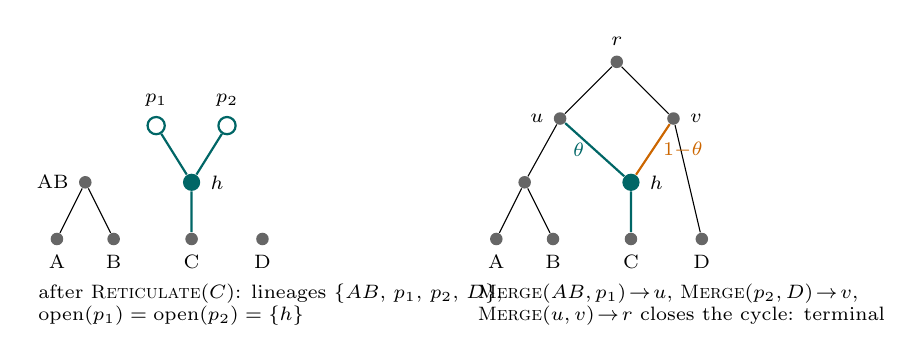
\begin{tikzpicture}[scale=0.9, every node/.style={font=\scriptsize}, dot/.style={circle,fill=black!60,inner sep=1.6pt}, ret/.style={circle,fill=teal!80!black,inner sep=2.2pt}, slot/.style={circle,draw=teal!80!black,thick,inner sep=2.2pt,fill=white}]
% state 2: reticulate C
\node[dot,label=below:A] (A) at (0,0) {}; \node[dot,label=below:B] (B) at (0.8,0) {}; \node[dot,label=below:C] (C) at (1.9,0) {}; \node[dot,label=below:D] (D) at (2.9,0) {};
\node[dot,label=left:AB] (AB) at (0.4,0.8) {}; \draw (AB)--(A) (AB)--(B);
\node[ret,label=right:$h$] (h) at (1.9,0.8) {}; \draw[teal!80!black,thick] (h)--(C);
\node[slot,label=above:$p_1$] (p1) at (1.4,1.6) {}; \node[slot,label=above:$p_2$] (p2) at (2.4,1.6) {};
\draw[teal!80!black,thick] (p1)--(h) (p2)--(h);
\node[align=left,anchor=north west] at (-0.4,-0.5) {after \textsc{Reticulate}$(C)$: lineages $\{AB,\,p_1,\,p_2,\,D\}$,\\ $\mathrm{open}(p_1)=\mathrm{open}(p_2)=\{h\}$};
% state 3
\begin{scope}[xshift=6.2cm]
\node[dot,label=below:A] (A) at (0,0) {}; \node[dot,label=below:B] (B) at (0.8,0) {}; \node[dot,label=below:C] (C) at (1.9,0) {}; \node[dot,label=below:D] (D) at (2.9,0) {};
\node[dot] (AB) at (0.4,0.8) {}; \draw (AB)--(A) (AB)--(B);
\node[ret,label=right:$h$] (h) at (1.9,0.8) {}; \draw[teal!80!black,thick] (h)--(C);
\node[dot,label=left:$u$] (u) at (0.9,1.7) {}; \draw (u)--(AB); \draw[teal!80!black,thick] (u)--(h) node[midway,left]{$\theta$};
\node[dot,label=right:$v$] (v) at (2.5,1.7) {}; \draw (v)--(D); \draw[orange!80!black,thick] (v)--(h) node[midway,right]{$1{-}\theta$};
\node[dot,label=above:$r$] (r) at (1.7,2.5) {}; \draw (r)--(u) (r)--(v);
\node[align=left,anchor=north west] at (-0.4,-0.5) {\textsc{Merge}$(AB,p_1)\!\to\!u$, \textsc{Merge}$(p_2,D)\!\to\!v$,\\ \textsc{Merge}$(u,v)\!\to\!r$ closes the cycle: terminal};
\end{scope}
\end{tikzpicture}
\end{center}

\paragraph{Trajectory length.} Each \textsc{Merge} removes one lineage, each \textsc{Reticulate} adds one; from $N$ lineages to $1$ with $R$ reticulations takes $N-1+R$ merges and $R$ reticulate actions: $N-1+2R$ steps (checked by \code{test\_trajectory\_length\_and\_reward}).

\subsection{The three masks and why there are no dead ends}
\begin{keybox}[Legality (constant time per action)]
\begin{itemize}[nosep]
\item \textsc{Merge}$(u,v)$ is legal iff $|\mathrm{open}(u)\cup\mathrm{open}(v)|\le1$ and $(u,v)$ are not the two bare slots of the same $h$.
\item \textsc{Reticulate}$(x)$ is legal iff $\mathrm{open}(x)=\emptyset$, fewer than $R_{\max}$ reticulations exist, and some \emph{other} lineage $y\neq x$ has $\mathrm{open}(y)=\emptyset$.
\end{itemize}
\end{keybox}
\emph{Why the first rule.} Merging two lineages that carry two different open reticulations $h\ne h'$ would create a node through which two cycles pass; in a binary network two cycles that share a vertex necessarily share an edge (a vertex of degree 3 cannot host two edge-disjoint cycles), which is level-2. Merging the two bare slots of one $h$ would create two parallel edges into $h$.

\emph{Why the second rule (no dead ends).} After \textsc{Reticulate}$(x)$ the slots $p_1,p_2$ cannot merge with each other and cannot merge with a lineage carrying a different open reticulation; they need a \emph{free} lineage ($\mathrm{open}=\emptyset$). The state $\{p_1,p_2,q_1,q_2\}$ (two bare pairs, nothing else) has no legal action at all. Requiring another free lineage at the moment of reticulating makes such states unreachable: by induction, every reachable non-terminal state has at least one legal action (if two free lineages exist, merge them; if one free and a pair, merge the free one into a slot; if only pairs, at least one pair is not bare, and its two carriers can close). The test \code{test\_class\_counts\_and\_no\_dead\_ends} enumerates \emph{all} reachable states for $N\le5$ and finds no dead end.

\emph{Why this is exactly the level-1 class.} Every terminal network is binary, acyclic (a new node is always older than what it connects) and level-1 (each cycle closes at exactly one reticulation and cycles are vertex-disjoint by the first rule). Conversely every level-1 network is reachable (induction on $R$: remove one cycle, build the rest, reticulate at the right moment). The enumeration in Part~VI confirms both directions numerically: the reachable terminal networks are $603=15+228+360$ for $N=4,R\le2$ and $11\,460=105+2\,805+8\,550$ for $N=5$, the published counts.

\subsection{Two features per lineage: the exact likelihood without $2^R$ trees}
\begin{keybox}[The trick]
A lineage $u$ that carries an open reticulation $h$ stores two Felsenstein features:
\begin{itemize}[nosep]
\item $A_u$ = feature of $u$ in the displayed trees where $u$'s side \emph{keeps} its edge into $h$;
\item $B_u$ = feature of $u$ in the displayed trees where that edge is \emph{deleted}.
\end{itemize}
For a bare slot: $A_{p_1}=\theta_h\,L_h$, $A_{p_2}=(1-\theta_h)\,L_h$, $B_{p_1}=B_{p_2}=\mathbf 1$ (all-ones: ``no data below'').\\
\textsc{Merge}$(u,v)\to w$ with lengths $(b_u,b_v)$, writing $T_u(\cdot)=(\cdot)\,P(b_u)^{\!\top}$:
{\small\begin{align*}
\text{both closed:}\ & A_w=T_u(A_u)\odot T_v(A_v);\\
\text{only $u$ open ($w$ stays open):}\ & A_w=T_u(A_u)\odot T_v(A_v),\quad B_w=T_u(B_u)\odot T_v(A_v);\\
\text{closing merge ($w$ closed):}\ & A_w=T_u(A_u)\odot T_v(B_v)+T_u(B_u)\odot T_v(A_v).
\end{align*}}
Edge priors $P(b)^{1/m}$ multiply both versions, exactly as in PhyloGFN.
\end{keybox}

\begin{proposition}\label{prop:mix}
For every level-1 network built by the MDP, the feature $A$ of the final lineage equals, at every site $i$, $\sum_{T\in\mathcal T(G)}w(T\mid\btheta)\,L^i_{\mathrm{root}}(\cdot\mid T,\bb)$ (times the edge priors). Hence $\sum_a\tfrac14A^i(a)$ is the network likelihood of site $i$ (eq.~\eqref{eq:netlik}).
\end{proposition}
\begin{proof}[Proof sketch]
Fix a reticulation $h$ with carriers $u$ (slot 1 side) and $v$ (slot 2 side) at the closing merge. The displayed trees split into those keeping $p_1$ (weight $\theta_h\cdot$rest) and those keeping $p_2$. In a tree keeping $p_1$, the edge $v\to h$ is deleted and the slot is suppressed, so $v$ contributes its feature \emph{without} the $h$ subtree: that is $B_v$ (the all-ones vector of a bare slot is invariant under $T_v$ because $P(b)\mathbf 1=\mathbf 1$, and suppressing a degree-2 node is exactly $P(b_1)P(b_2)=P(b_1+b_2)$). Symmetrically for trees keeping $p_2$. Because pruning is linear in each child feature and $\theta_h,1-\theta_h$ were folded into $A_{p_1},A_{p_2}$, the sum of the two products is the $\theta$-weighted sum over the two families of displayed trees. Cycles of a level-1 network are vertex-disjoint, so the families of different reticulations are independent and the argument applies to each closing merge in turn; nested (closed) cycles enter as already-mixed features, by linearity.
\end{proof}
The test \code{test\_likelihood\_matches\_explicit} compares this with an explicit enumeration of all $2^R$ displayed trees (\file{src/utils/network\_likelihood.py}) on random networks with up to 7 leaves and 3 reticulations; the largest difference is $1.5\times10^{-11}$.

\begin{whybox}[Why this matters for scalability]
The naive network likelihood costs $2^R$ Felsenstein passes; ours costs \emph{one} pass with at most two vectors per lineage --- $O(N\,m\,|\Sigma|^2)$ per trajectory, the same order as a tree. This is what makes reward evaluation compatible with the ``reward is the dominant per-trajectory cost'' analysis of the proposal.
\end{whybox}

\subsection{Ordering keys: keeping the list sorted so that actions are reproducible}
PhyloGFN sorts subtrees by their smallest leaf index. A bare slot has no leaves, and the leaves below $h$ would be counted by \emph{both} sides of $h$. We therefore give every lineage a set of \emph{tokens}: the leaf indices $0,\dots,N-1$, plus one fresh token $N+\mathrm{id}(h)$ for slot 2 of every reticulation; slot 1 inherits the tokens of $h$'s child. Tokens partition a set, so the minimum token (the \emph{key}) of each lineage is unique and the sorted-by-key list is well defined. \textsc{Merge}$(i<j)$ places the new lineage at position $i$; \textsc{Reticulate}$(i)$ places $p_1$ at position $i$ and appends $p_2$ (its fresh token is larger than every other key). The backward sampler recomputes action indices by replaying forward under this convention (\code{test\_backward\_sampling\_roundtrip}).

\subsection{Backward policy: counting parents correctly}
$|\mathrm{Pa}(s')|=$ (number of real lineages whose root is a tree node: undo a merge) $+$ (number of reticulations whose two slots are both bare in $s'$, \emph{provided $s'$ contains a free lineage}: undo a reticulation). The proviso is essential: undoing \textsc{Reticulate}$(x)$ leads to a state from which \textsc{Reticulate}$(x)$ is legal only if another free lineage exists; without the proviso we would count a ``parent'' that is not in the state graph, and $\PB$ would not be a distribution over actual parents --- the TB identity would be silently wrong. At the terminal state (rooted network) there is exactly one parent, the un-merge of the root; we keep the terminal object \emph{rooted} (reticulations are directed, so the root is meaningful), unlike PhyloGFN's unrooted trees with $2N-3$ last-step parents.

\subsection{Priors}
$p(\bb)=\prod_e\lambda e^{-\lambda b_e}$ with PhyloGFN's root convention (the two root edges count as one edge of length $b_l+b_r$); $p(\theta_h)=\mathrm{Uniform}(0,1)$. For the topology two priors are implemented (config \code{PRIOR\_TYPE}):
\begin{itemize}[nosep]
\item \code{EXP\_R} (the proposal's formula): $p(G)\propto e^{-\lambda_RR(G)}$ over the level-1 class, $R\le R_{\max}$;
\item \code{UNIFORM\_R}: $p(R)\propto e^{-\lambda_RR}$ and, given $R$, uniform over the $r(N,R)$ topologies: $\log p(G)=-\lambda_RR-\log r(N,R)+\text{const}$.
\end{itemize}
The difference is not cosmetic. The class sizes grow fast with $R$: for $N=6$, $r(6,1)/r(6,0)=41.6$ and $r(6,2)/r(6,1)=5.0$; for $N=27$ the ratios are in the thousands. Under \code{EXP\_R} the prior mass of ``some $R$'' is $r(N,R)e^{-\lambda_RR}$, so with $\lambda_R=1$ a 6-taxon prior already favours $R=2$ over $R=1$ by $1.8:1$ and $R=1$ over $R=0$ by $15:1$ \emph{before seeing any data}. \code{UNIFORM\_R} removes the class-size effect and makes $\lambda_R$ a genuine penalty per reticulation ($p(R)\propto e^{-\lambda_R R}$). Both are exact in the code; the normaliser needed for the MLL estimate uses the exact counts $r(N,k)$ in the first case and $\sum_k e^{-\lambda_Rk}$ in the second. Because $\log p(G)$ is added to $\log\R$, the sampler's marginal over $R$ is a genuine posterior over the number of reticulations under the chosen prior.

\subsection{The policy for two kinds of action}
The Transformer sees, per lineage, $[\,\bar A\,;\,\bar B\,;\,\text{4 flags}\,]$ where $\bar A,\bar B$ are the per-site normalised features (as PhyloGFN normalises $\rho$) and the flags are (has open reticulation, is bare slot, which side of $h$, its inheritance share $\theta$ or $1-\theta$). The flags let the policy recognise the two carriers of the same $h$ (their $A$ vectors share the $h$-subtree pattern). The action logits are the concatenation $[\text{pair logits}\mid\text{single logits}]$: pairs from the PhyloGFN head on $e_i+e_j$, singles from a new head on $e_i$; illegal entries are set to $-\infty$ using the environment's mask; $\varepsilon$-exploration picks a uniformly random \emph{legal} action. A \textsc{Reticulate} action then draws $(\log b_{hx},\mathrm{logit}\,\theta_h)$ from a 2-D Gaussian mixture (new head) with the change of variables $\log p(\theta)=\log p(\mathrm{logit}\,\theta)-\log\theta-\log(1-\theta)$.

\subsection{Variable-length batches}
Trajectories in a batch no longer share a step index, so the rollout worker keeps a \code{done} mask, runs the policy only on active trajectories, pads the lineage dimension to $l_{\max}=N+R_{\max}$ (the Transformer already supports padding masks) and accumulates $\sum\log\PF$ and $\sum\log\PB$ per trajectory as it goes. The TB loss is then identical in form to PhyloGFN's.
\clearpage
